\documentclass{article}

\usepackage[utf8]{inputenc}
\usepackage{amssymb}
\usepackage{amsmath}
\usepackage{float}
\usepackage{latexsym}
\usepackage{subcaption}
\usepackage{gensymb}
\usepackage{caption}
\usepackage{fancyhdr}
\usepackage{lastpage}
\usepackage{extramarks}
\usepackage[usenames,dvipsnames]{color}
\usepackage{graphicx}
\usepackage{listings}
\usepackage{courier}
\usepackage{lipsum}
\usepackage{tabularx}
\usepackage{color}

\definecolor{mygreen}{rgb}{0,0.6,0}
\definecolor{mygray}{rgb}{0.5,0.5,0.5}
\definecolor{mymauve}{rgb}{0.58,0,0.82}

\lstset{
  backgroundcolor=\color{white},   
  breaklines=true,
  captionpos=b,
  commentstyle=\color{mygreen},
  escapeinside={\%*}{*)},
  extendedchars=true,
  frame=single,
  keepspaces=true,
  keywordstyle=\color{blue},
  language=Octave,
  otherkeywords={*,...},
  numbers=left,
  numbersep=5pt,
  numberstyle=\tiny\color{mygray},
  rulecolor=\color{black},
  showspaces=false,
  showstringspaces=false,
  showtabs=false,
  stepnumber=2,
  stringstyle=\color{mymauve},
  tabsize=2,
  title=\lstname
}

\topmargin=-0.45in
\evensidemargin=0in
\oddsidemargin=0in
\textwidth=6.5in
\textheight=9.0in
\headsep=0.25in
\linespread{1.1} % Line spacing


\chead{}
\lfoot{\lastxmark} % Bottom left footer
\cfoot{} % Bottom center footer
\rfoot{Page\ \thepage} % Bottom right footer
\renewcommand\headrulewidth{0.4pt} % Size of the header rule
\renewcommand\footrulewidth{0.4pt} % Size of the footer rule
\setlength\parindent{16pt} % Removes all indentation from paragraphs
\setcounter{secnumdepth}{0} % Removes default section numbers
\title{
\vspace{1in}
\textmd{\textbf{Advanced Topics in Machine Learning - Assignment 7}} \\
\author{Christoffer Thrysøe - dfv107}
}

\begin{document}
\maketitle
\pagenumbering{arabic}
\section{1 Label-efficient prediction and label-efficient bandits}
\subsection{1.1}
We have that $Z_t$ is a Bernoulli random variable with bias $\varepsilon$, therefore the probability is given by:
\begin{align*}
P\lbrace Z_t &= 1 \rbrace = \varepsilon \\
P\lbrace Z_t &= 0 \rbrace = 1-\varepsilon \\
\end{align*}
The expected value $Z_t$ is given as followed:
\begin{equation}
\mathbb{E}[Z_t] = P\lbrace Z_t = 1 \rbrace \cdot 1 + P\lbrace Z_t = 0 \rbrace \cdot 0 = \varepsilon \cdot 1 + (1- \varepsilon) \cdot 0 = \varepsilon
\end{equation}
Thus the expected value of $Z_t$ is it's bias $\varepsilon$. For the algorithm, we draw $Z_t$ at each iteration. We wish to express how many times we can expect to have $Z_t = 1$ over the $T$ iterations. To quantify this, we sum the expected value, which we just derived:
\begin{align}
\mathbb{E} \left[ \sum\limits_{t=1}^T Z_t \right] = \sum\limits_{t=1}^T  \mathbb{E}[ Z_t] = \sum\limits_{t=1}^T  \varepsilon = \varepsilon T
\end{align}
where the second term follows from the linearity of expectation, which allows us to move the expected value into the sum. Thus concluding that the expected number of times the algorithm requests to observe the labels is $\varepsilon T$.
\subsection{1.2}
For the algorithm, we are in adversarial full information setting. That is, when we request to observe the columns, we are allowed to observe $l_t^1 .\dots, l_t^K$. We wish to show that the expected regret of the algorithm satisfies the following bound on the expected regret:
\begin{equation}
\mathbb{E}[R_T] \leq \sqrt{2 \frac{1}{\varepsilon} T \ln K}
\end{equation}
 If we have that $\varepsilon = 1$, we recover the exact same algorithm as hedge, I will therefore use a similar approach to bounding the expected regret. The initial analysis is similar to the hedge, therefore I will start by lemma 5.2 from Yevgeny's lecture notes and work from there. 
The lemma states:
\begin{equation}
\label{eq:12}
\sum\limits_{t=1}^T\sum\limits_{a=1}^K p_t(a) l_t^a - \min_a L_T(a) \leq \dfrac{\ln K}{\eta} + \dfrac{\eta}{2} \sum\limits_{t=1}^T\sum\limits_{a=1}^K p_t(a) (l_t^a)^2
\end{equation}
First we note that the left hand side of \eqref{eq:12} is the expected regret. We only observe and record loss if $Z_t=1$, which we from the previous assignment know is expected to happen $\varepsilon T$ times, thus we only need to sum $\varepsilon T$ times instead of $T$ times.  We also note that since our loss is scaled with $\varepsilon$, that is from the algorithm. when we update our loss, we take $l_t^a / \varepsilon$ and since $l_t^a \in [0,1]$, we know that for our algorithm, the added loss will be $\l_t^a \in [0,\frac{1}{\varepsilon}]$
Thus we can write the following:
%, thus if we take out a single loss from \eqref{eq:12} and denote it $1/\varepsilon$ we get:
\begin{align}
\dfrac{\ln K}{\eta} + \dfrac{\eta}{2} \sum\limits_{t=1}^{\varepsilon T}\sum\limits_{a=1}^K p_t(a) (l_t^a)^2 &\leq
\dfrac{\ln K}{\eta} + \dfrac{\eta}{2} \sum\limits_{t=1}^{\varepsilon T}\sum\limits_{a=1}^K \left( \dfrac{1}{\varepsilon}\right)^2 p_t(a) \\
&\leq \dfrac{\ln K}{\eta} +  \dfrac{\eta}{2} \sum\limits_{t=1}^{\varepsilon T} \dfrac{1}{\varepsilon^2} \\
&= \dfrac{\ln K}{\eta} +  \dfrac{\eta}{2} \dfrac{T}{\varepsilon} \\
&= \dfrac{\ln K}{\eta} + \dfrac{\eta T}{2 \varepsilon}
\label{eq:her}
\end{align}
Taking the derivative with respect to $\eta$ we get:
\begin{equation}
\dfrac{\partial}{\partial \eta} \left[ \dfrac{\ln K}{\eta} + \dfrac{\eta T}{2 \varepsilon} \right] = - \dfrac{\ln k}{\eta^2} + \dfrac{T}{2 \varepsilon}
\end{equation}
Setting the derivative to zero:
\begin{align}
0 &= - \dfrac{\ln k}{\eta^2} + \dfrac{T}{2 \varepsilon} \Rightarrow \\
\eta &= \sqrt{\dfrac{2 \varepsilon \ln K}{T}}
\label{eq:opt}
\end{align}
The second derivative of \eqref{eq:her} is $\dfrac{2 \ln k}{\eta^3}$ and since $\eta$ is positive, we have that the optimum in \eqref{eq:opt} is an extremal point. Setting this optimal value for $\eta$ in \eqref{eq:her} we get the following:
\begin{align}
\dfrac{\ln K}{\eta} + \dfrac{\eta}{2 \varepsilon} T &=\dfrac{\ln K}{\sqrt{\dfrac{2 \varepsilon \ln K}{T}}} + \dfrac{T \sqrt{\dfrac{2 \varepsilon \ln K}{T}}}{2 \varepsilon} \\
&= \sqrt{2 \ln K \frac{T}{\varepsilon}}
= \sqrt{2 \frac{1}{\varepsilon} T  \ln K }
\end{align}
From \eqref{eq:12} we now have that 
\begin{equation}
\mathbb{E}[R_T] \leq \sqrt{2 \frac{1}{\varepsilon} T  \ln K }
\end{equation}

which is what we wanted to prove.
\subsection{1.3}
We wish to show that with high probability the exact number of observed columns is not significantly larger than $\varepsilon T $. That is we wish to provide a bound on the probability that the sum of our independent random variable $Z_t$ deviates from its expected value $\varepsilon T$. For this we can use Hoeffding's inequality, which is listed in Corollary 2.4 in Yevgeny's lecture notes:
\begin{equation}
P \left\lbrace \dfrac{1}{T} \sum\limits_{i=1}^T Z_t - \mathbb{E}[Z_t] \geq \epsilon \right \rbrace \leq e^{-2 T \epsilon^2}
\end{equation}
If we take $\epsilon = \sqrt{\frac{\ln \frac{1}{\delta}}{2T}}$ we get:
\begin{equation}
\label{eq:probbound}
P \left\lbrace \dfrac{1}{T} \sum\limits_{i=1}^T Z_t - \mathbb{E}[Z_t] \geq \sqrt{\dfrac{\ln \frac{1}{\delta}}{2T}} \right \rbrace \leq \delta
\end{equation}
To get a high probability bound, we re-write \eqref{eq:probbound}:
\begin{align}
P \left\lbrace \dfrac{1}{T} \sum\limits_{i=1}^T Z_t - \mathbb{E}[Z_t] \leq \sqrt{\dfrac{\ln \frac{1}{\delta}}{2T}} \right \rbrace \geq 1- \delta \\
P \left\lbrace \dfrac{1}{T} \sum\limits_{i=1}^T Z_t \leq  \dfrac{1}{T} \sum\limits_{i=1}^T \mathbb{E}[Z_t] + \sqrt{\dfrac{\ln \frac{1}{\delta}}{2T}} \right \rbrace \geq 1- \delta
\label{eq:ineq}
\end{align}
Thus, with high probability $1 - \delta$, we have that exact number of observed columns is not significantly higher than $\varepsilon T$. If it was significantly higher, then the first inequality of \eqref{eq:ineq}, would not hold.
\subsection{1.4}
\subsection{1.5}
%http://www.ii.uni.wroc.pl/~lukstafi/pmwiki/uploads/AGT/Prediction_Learning_and_Games.pdf
% 131
\section{2 Policy evaluation}
We wish to prove that the iterative policy evaluation converges to the true value function, that is: $\forall s \in S : \lim_{k\rightarrow \infty} V_k(s) = V^\pi(s)$, where the update rule is given by:
\begin{equation}
\forall s \in S : V_{k+1}(s) \leftarrow \sum\limits_a \pi(s,a) \sum\limits_{s'} P^a_{ss'} [ R^a_{ss'} + \gamma V_k(s')]
\end{equation}
and  $0 < \gamma < 1$. First we note that for the converged value function we have:
\begin{equation}
V^\pi(s) = \sum\limits_a \pi(s,a) \sum\limits_{s'} P^a_{ss'} [ R^a_{ss'} + \gamma V^\pi(s')]
\end{equation}
We note, by definition that:
\begin{align}
V_{k+1} &= \sum\limits_a \pi(s,a) \sum\limits_{s'} P^a_{ss'} [ R^a_{ss'} + \gamma V_k(s')] \\
&\leq \sum\limits_a \pi(s,a) \sum\limits_{s'} P^a_{ss'} [ R^a_{ss'} + \gamma V^\pi(s')] \\
&= V^\pi(s)
\end{align}
and we define:
\begin{align}
\label{eq:max}
\Delta_k &= \max_s | V_k(s) - V^\pi(s)|
\end{align}
rewriting \eqref{eq:max}, we define:
\begin{equation}
\label{eq:newdif}
V_k(s) \geq V^\pi(s) - \Delta_k
\end{equation}
Now we can write:
\begin{align}
V_{k+1} &= \sum\limits_a \pi(s,a) \sum\limits_{s'} P^a_{ss'} [ R^a_{ss'} + \gamma V_k(s')] \\
&\geq \sum\limits \pi (s,a) \sum_{s'} P^a_{ss'} [R^a_{ss'} + \gamma(V^\pi(s') - \Delta_k)] \\
&= \sum\limits \pi (s,a) \sum_{s'} P^a_{ss'} [R^a_{ss'} + \gamma(V^\pi(s')] - \sum\limits_a \pi(s,a) \sum\limits_{s'} P^a_{ss'} \gamma \Delta_k
\end{align}
where the above follows from \eqref{eq:newdif} and taking $\Delta_k$ outside. We note that $\sum_{s'}P^a_{ss'} = 1$ and therefore we can get the following:
\begin{align}
\sum\limits_a \pi (s,a) \sum\limits_{s'} P^a_{ss'} [R^a_{ss'} + \gamma(V^\pi (s')] - \sum\limits_{a} \pi (s,a) \sum\limits_{s'} P^a_{ss'} \gamma \Delta_k &= V^\pi (s) - \sum\limits_{a} \pi (s,a) \gamma \Delta_k \\
&\geq V^\pi (s) - \gamma \Delta_k
\end{align}
where the last line holds because $\pi(s,a) \leq 1$. Thus we have that:
\begin{align}
\sum\limits \pi (s,a) \sum_{s'} P^a_{ss'} [R^a_{ss'} + \gamma(V^\pi(s') - \Delta_k)] \geq V^\pi (s) - \gamma \Delta_k \Leftrightarrow V^\pi(s) - \Delta_k \geq V^\pi(s) - \gamma \Delta_k
\end{align}
which implies that:
\begin{equation}
\Delta_{k+1} \leq \gamma \Delta_k
\end{equation}
Because of the above, we can now state the following:
\begin{equation}
| V_{k+1}(s) - V^\pi(s)| \leq \gamma | V_k(s) - V^\pi(s) | \leq \dots \leq \gamma^{k+1} | V_{0}(s) - V^\pi(s)|
\end{equation}
with $0 < \gamma < 1$. Because the difference converges to zero, $V_k(s)$ converges towards $V^\pi(s)$, thus concluding that: 
\begin{equation}
\lim_{k \rightarrow \infty} V_k(s) = V^\pi(s)
\end{equation}
which is what we wanted to prove.
\\
\\
\\
\begin{align}
| V_{k+1}(s) - V^\pi(s) | &=  \left| \sum\limits_a \pi(s,a) \sum\limits_{s'} P^a_{ss'} [ R^a_{ss'} + \gamma V_k(s')]  - \sum\limits_a \pi(s,a) \sum\limits_{s'} P^a_{ss'} [ R^a_{ss'} + \gamma V^\pi(s')] \right| \\
&= \sum\limits\limits_a \pi (s,a) \sum\limits_s' ( | P_{ss'}^a R_{ss'}^a + \gamma P_{ss'}^a V_k(s') - P_{ss'} R_{ss'}^a - \gamma P_{ss'}^a V^\pi (s'))| \\
&= \sum\limits_a \pi(s,a) \sum\limits_{s'} \gamma P_{ss'}^a (|V_k(s') - V^\pi(s')|) \\
&\leq \sum\limits_a \pi(s,a) \sum\limits_{s'} \gamma (|V_k(s') - V^\pi(s')|) \\
&= \sum\limits_a \pi (s,a) \sum\limits_{s'} \gamma ( \sum\limits_a \pi (s,a) \sum\limits_{s'} \gamma P_{ss'}^a ( V_{k-1}(s') - V^\pi (s'))
\end{align}


\section{3 Reinforcement learning}
For this assignment, we have been given a floor plan, which represents an apartment with $3\times4=12$ rooms. Each room has at least one door, which the agent can use to enter the adjacent room (if connected by a door), and some rooms may contain a penalty when entered. Each move done by the agent will inflict a penalty -1. The agent has four possible movements at each state: $\lbrace \text{up,down,right,left} \rbrace$. If the agent chooses an action, where there is no door to connect to the next room, the agent will remain in the same room, viewed as the agent bumping into the door-less wall. When bumping into a wall, the movement penalty of -1 is still enforced. In the apartment, there is a single room, which is a terminal state. When entered, the episode ends and the agent does not move further. 
The problem was modelled using an \texttt{Apartment} object, which keeps track of each room in the apartment and is used to fetch a given room and set the initial rewards and so on. An object for \texttt{Room} is also used, which is a model for each room i.e. state in the apartment. Each room contains information such as room number, the reward of the room (which in our case is only negative), the action policy of the room $\pi(s,a)$, which is the probability of performing action $a$ when being in state $s$, and a mapping of each action to a new state. For example for room 0 (the upper left room) the "\texttt{up}" action maps to going into a wall (which i denote -1 to identify), as there is no door going up. The "\texttt{right}" action maps to room 1 (which is to it's right, connected by a door).
\subsection{3.1}
We wish to implement a Markov decision process (MPD) to compute the value function $V^{rand}$. $rand$ means that the policy is uniform. Therefore for each possible action, in each state, the policy, i.e. the probability of performing an action given a state, will be uniform: $\pi(s_i,a_j) = 0.25$ because at each state the agent has four possible actions. For this task I have chosen to implement the iterative policy evaluation algorithm, which is shown in algorithm 1. 
\begin{figure}[H]
  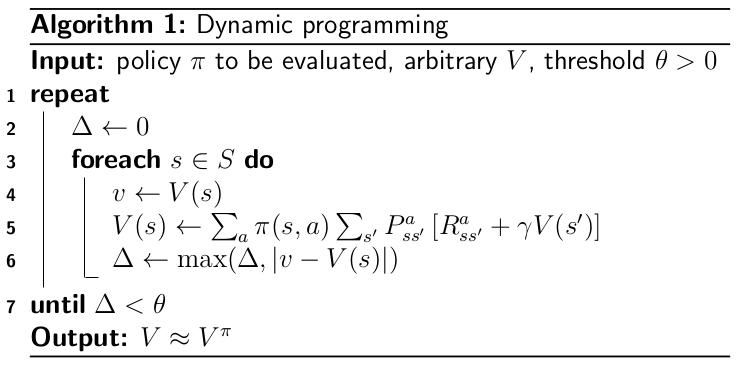
\includegraphics[width=9cm]{fig/1.png}
\end{figure}
$P^a_{ss'}$ is the probability of going to state $s'$ when being in state $s$ and performing action $a$. For this given problem, the probability will be $1$ or $0$, because the transitions are deterministic e.g. if we are in room 0 and choose the action "\texttt{right}", we will with probability 1 go to room 1, thus for the calculation on line 5 in algorithm 1, we only need to sum up rewards for each possible actions. The reward $R^a_{ss'}$ is also deterministic, where we enforce a penalty of -1 for each movement and entering certain rooms give a greater penalty. However if the agent is in one of the extra penalized rooms and bump into a wall, this penalty is not enforced again, only the penalty of -1 for making a move. The terminal state was implemented such that no penalty was made when moving inside, i.e. bumping into a wall when being in the terminal state, and the agent could not leave the state. The algorithm was run with $\gamma =1.0$, which is a setting we can chose since we have a zero reward absorbing state (terminal state), which is reachable from all states. The algorithm also takes an initial value function $V$ with all it's entries set to zero. The stopping criteria was set to $\theta = 1 \times 10^{-13}$. The returned value function $V^{rand}$, after running the algorithm was:
\begin{equation}
\label{eq:V1}
V^{rand} = \begin{bmatrix}
-224 & -218 & -218 \\
-226 & -203 & -214 \\
-214 & -184 & -201 \\
-228 & -94 & 0
\end{bmatrix}
\end{equation}
where the entries in the matrix corresponds to the given room, i.e the value for room 0 is $-224$. As evident from \eqref{eq:V1}, the worst starting place is room 9, which is because we must go through room 6, which has a penalty of -10. The lowest penalty (not including the terminal state) is room 10, which is adjacent to the terminal state.
\subsection{3.2}
For this assignment we wish to compute the optimal value function $V^*$, that is at each state we want to find the optimal action, which is the action that gets us with least penalty to the terminal state. To solve this, I have implemented the policy iteration algorithm, shown in algorithm 2.
\begin{figure}[H]
  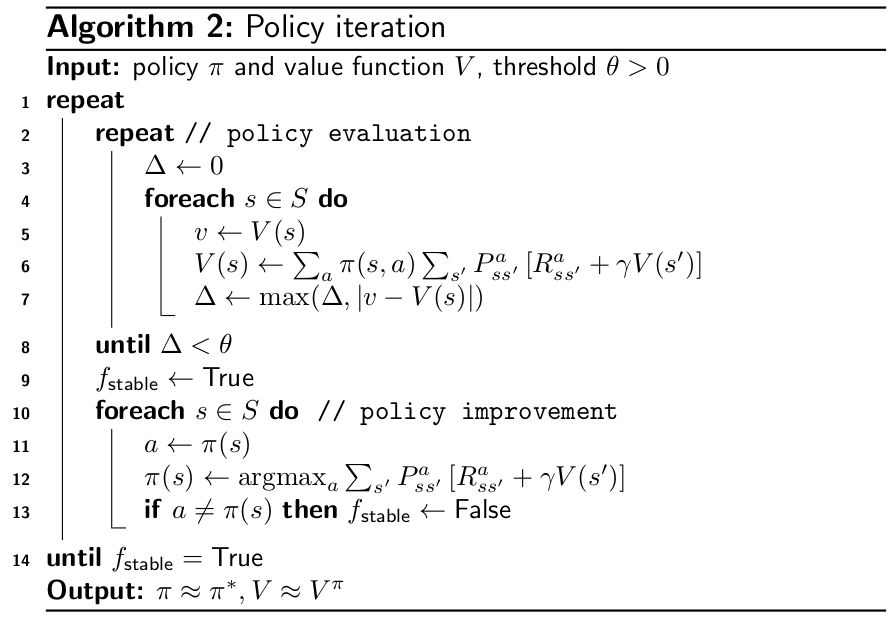
\includegraphics[width=10cm]{fig/5.png}
\end{figure}
The algorithm consists of two steps, the first step is evaluating the value function $V^\pi$ based on the given policy $\pi$, in which we can use the algorithm presented in question 3.1. The next step is checking to see if we can improve this policy. If it can be improved, we start over and compute the value function again with the new improved policy $\pi$. If we can't further optimize the policy, we terminate with the given policy $\pi^*$ and value function $V^\pi$. For the algorithm I started out with the uniform probability for each action modelled as a list $[0.25, 0.25, 0.25, 0.25]$. As evident from line 12 in algorithm 2, the algorithm chooses a new single action which optimizes the reward, for example if the was action "\texttt{up}", it is represented as $[1,0,0,0]$, which is because $\pi$ can map a state and an action to a probability or it can map a state to a given action, this way of representing the policy allows me to do both. Running the algorithm gives an optimal policy for each state and a value function, first I will show the policy and then the Value function. 
Figure \ref{fig:1} shows the apartment and the numbering of each room. The arrows represent the action of the optimal policy, returned from algorithm 2. Looking at the arrows, they all make sense with regards to getting to the Terminal state with as little penalty as possible. For example if we take room 3: The shortest path may be to move down instead of up, but because a penalty of 10 is enforced by moving down it moves up resulting in a total penalty of 11 instead of 14.
\begin{figure}[H]
\centering
  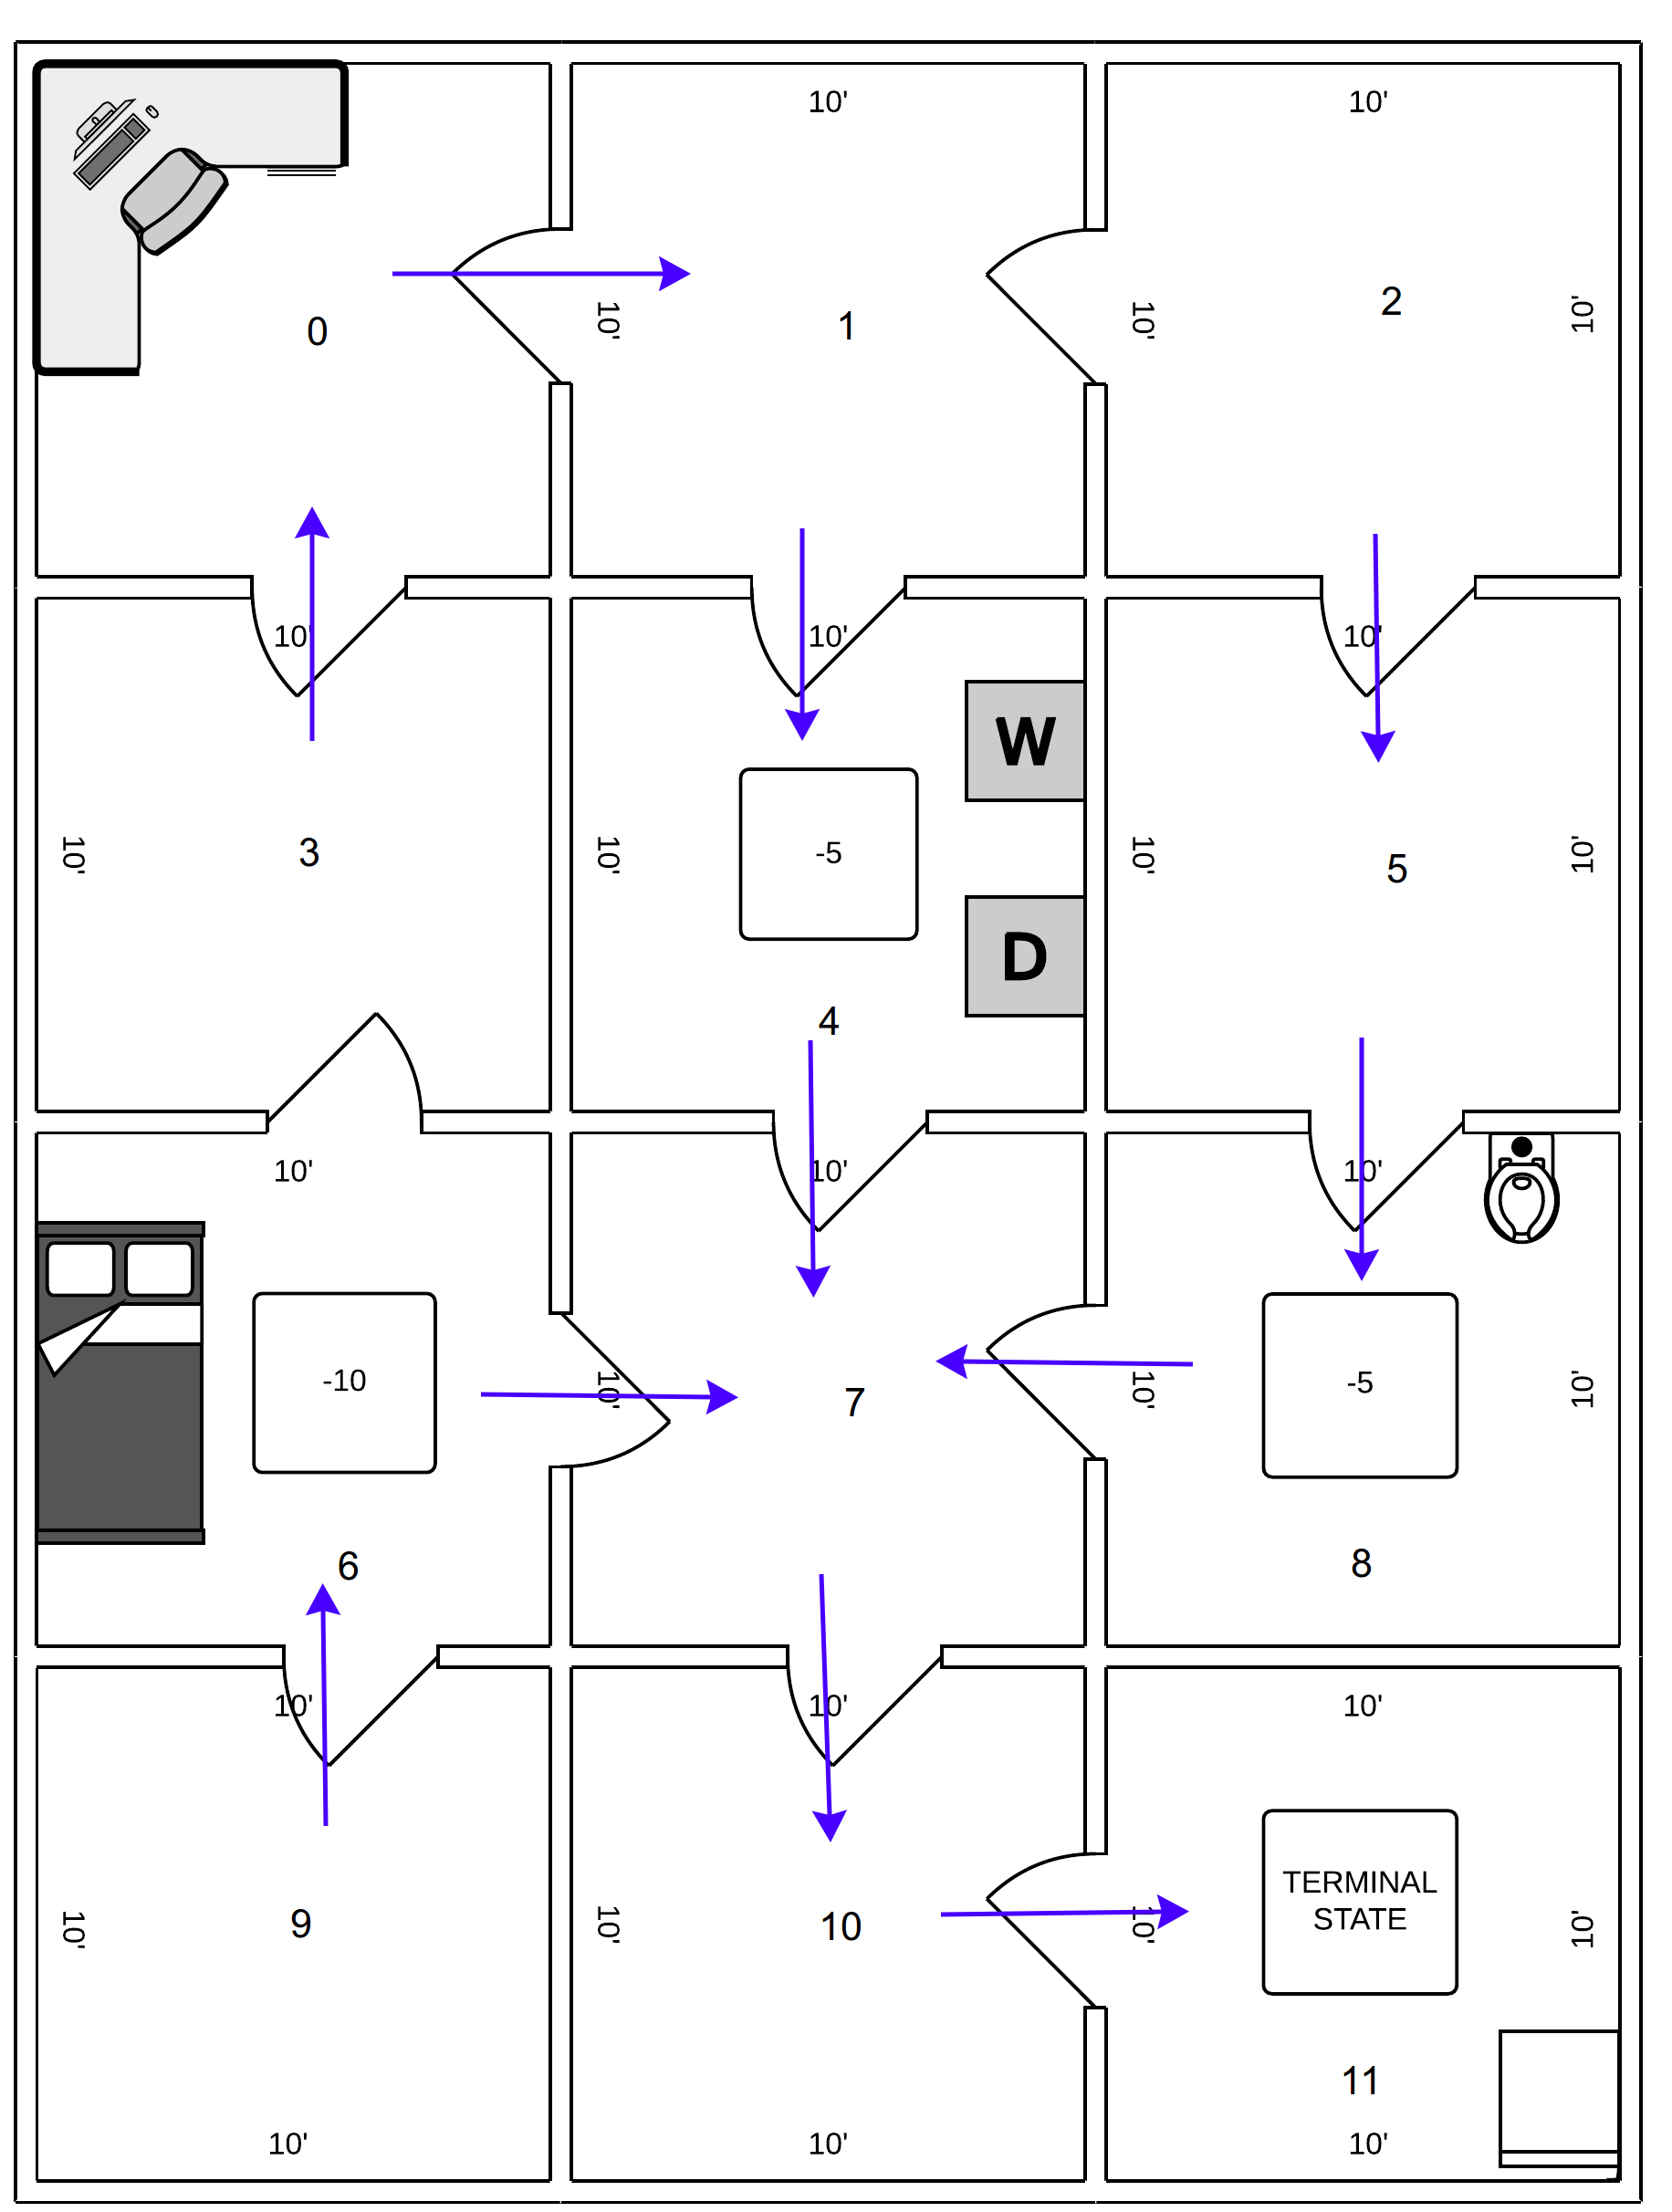
\includegraphics[width=8cm]{fig/apartment.png}
\caption{\label{fig:1} The returned optimal policy returned from algorithm 2. The arrows represent the optimal action for each state, e.g. the optimal action for room 5 is down.}
\end{figure}

The return value function $V^*$ is given as followed:
\begin{equation}
V^* = 
\begin{bmatrix}
-10 & -9 & - 10 \\
-11 & -3 & -9 \\
-3 & -2 & -3 \\
-14 & -1 & 0
\end{bmatrix}
\end{equation}
This value function can easily be verified by looking at figure \ref{fig:1}, following the arrows from each state and counting the accumulated penalty, before reaching the terminal state. As with the random policy,  the worst starting location is at room 9.
\section{4 Bonus: Make Your Own Question}
My proposed question is about support vector machines and the use of the dual representation of the optimization problem. I have chosen this question as I found it difficult to understand the different representations of the problem and the benefits of using these representations.  This question will provide some "hands on" experience with the dual representation of the SVM optimization problem.
%pay much attention to the dual formulation of the SVM problem and this will give hands on experience with working with the dual representation.\\
\subsection{Question:}
%http://www.stolerman.net/studies/cs613/cs613_hw3_sol.pdf
Use the dual representation of the SVM optimization problem to show that regardless of the feature space dimensionality of the data, we can determine a hyperplane using only two points, having different class labels:
\begin{align}
x_1 &\in C_1,(y_1 = +1) \\
x_2 &\in C_2, (y_2 = -1)
\end{align}
That is we have:
\begin{align}
y(x_1) &= w^T x_1 + b = +1 \\
y(x_2) &= w^T x_2 + b = -1
\end{align}
The dual problem is defined as:
\begin{align}
\label{eq:q}
\text{Maximize}_\alpha \hspace{0.5cm}& \sum\limits_{i=1}^N \alpha_i - \frac{1}{2} \sum\limits_{i,j=1}^N \alpha_i \alpha_j y_i y_j \langle x_i, x_j \rangle \\
\text{subject to} \hspace{0.5cm}& \sum\limits_{i=1}^N \alpha_iy_i = 0 \\
 \hspace{0.5cm}& \alpha_i \geq 0 ,i =1,...,N
\end{align}
With $N=2$ we can reformulate the constraints as:
\begin{align}
\alpha_1 - \alpha_2 &= 0 \\
\alpha_1,\alpha_2 &\geq 0
\end{align}
The rest of the proof would consist of writing out the sums of the dual problem listed in \eqref{eq:q} for the two points. Then taking the derivative with respect to $\alpha$ (for $\alpha_1,\alpha_2$), setting them to zero and getting both $\alpha$. Once these have been expressed, they can be used to solve for the hyperplane using the following:
\begin{equation}
w = \sum\limits_{i=1}^N \alpha_i y_i x_i
\end{equation}
and solving for $b$:
\begin{equation}
b = - \dfrac{\max_{y_i = -1} ( \langle w,x_i \rangle ) + \min_{y_i=1} ( \langle w,x_i \rangle )}{2}
\end{equation}
where we know that the two data points are the support vectors.
\end{document}
